% AEJ-Article.tex for AEA last revised 22 June 2011
\documentclass[PP]{AEA}

%%%%%% NOTE FROM OVERLEAF: The mathtime package is no longer publicly available nor distributed. We recommend using a different font package e.g. mathptmx if you'd like to use a Times font.
\usepackage{mathptmx}

% The mathtime package uses a Times font instead of Computer Modern.
% Uncomment the line below if you wish to use the mathtime package:
%\usepackage[cmbold]{mathtime}https://www.overleaf.com/project/5de54d6638f785000167866a
% Note that miktex, by default, configures the mathtime package to use commercial fonts
% which you may not have. If you would like to use mathtime but you are seeing error
% messages about missing fonts (mtex.pfb, mtsy.pfb, or rmtmi.pfb) then please see
% the technical support document at http://www.aeaweb.org/templates/technical_support.pdf
% for instructions on fixing this problem.

% Note: you may use either harvard or natbib (but not both) to provide a wider
% variety of citation commands than latex supports natively. See below.

% Uncomment the next line to use the natbib package with bibtex 
\usepackage{url}
\urlstyle{same} % makes the font the same
\usepackage{natbib}
\usepackage{hyperref}
\usepackage{acronym}
\usepackage[names]{xcolor}
\usepackage{graphicx}
\usepackage{csvsimple}
% Uncomment the next line to use the harvard package with bibtex
%\usepackage[abbr]{harvard}
\usepackage{etoolbox}
\usepackage{geometry}
\usepackage{caption} % to re-use counters
\usepackage{threeparttable}

\newtoggle{fancy}
\togglefalse{fancy}

\newtoggle{draft}
%\toggletrue{draft}
\togglefalse{draft}

\newtoggle{final}
\togglefalse{final}
%\toggletrue{final}
%\iftoggle{final}{\togglefalse{draft}}{}


\iftoggle{draft}{
\usepackage{draftwatermark}
\SetWatermarkText{DRAFT}
\SetWatermarkScale{0.5}
\SetWatermarkLightness{0.85}%
}{\usepackage[final]{draftwatermark}}

\usepackage{xspace}
% to adjust floats
\usepackage{placeins}
% to read the table
\usepackage{booktabs}
\usepackage{ifthen}
\usepackage{csvsimple}
\usepackage{longtable}

\usepackage{textcomp}


\iftoggle{final}{
\usepackage[disable]{todonotes}
\newcommand{\misscitep}[2]{\citep{#2}}
\newcommand{\misscitet}[2]{\citet{#2}}
}{
\usepackage{todonotes}
\geometry{verbose,letterpaper,
	tmargin=1in,bmargin=1in,lmargin=1in,rmargin=2in}
\setlength{\marginparwidth}{1.9in}
\newcommand{\misscitep}[2]{\todo[color=green]{Missing citation: #1}{(\textcolor{red}{#2})}}
\newcommand{\misscitet}[2]{\todo[color=green]{Missing citation: #1}{\textcolor{red}{#2}}}
}



% This command determines the leading (vertical space between lines) in draft mode
% with 1.5 corresponding to "double" spacing.
\draftSpacing{1.5}

%% make somewhat tigher enumeration environments
\usepackage{enumitem}
\setlist[enumerate]{itemsep=0pt,parsep=0pt,topsep=1pt}
\setlist[itemize]{itemsep=0pt,parsep=0pt}

%% Acronyms
\acrodef{AEA}{American Economic Association}
\acrodef{AJPS}{American Journal of Political Science}
\acrodef{BPLIM}{Banco de Portugal Microdata Research Laboratory}
\acrodef{BLS}{Bureau of Labor Statistics}
\acrodef{CJE}{Canadian Journal of Economics}
\acrodef{CSWEP}{AEA Committee on the Status of Women in the Economics Profession}
\acrodef{DCAP}{data and code availability policy}
\acrodef{DOI}{Digital Object Identifier}
\acrodef{EJ}{Economic Journal}
\acrodef{FAIR}{Findable, Accessible, Interoperable, Re-usable}
\acrodef{FAQ}{frequently asked questions}
\acrodef{FSRDC}{Federal Statistical Research Data Centers}
\acrodef{HRS}{Health and Retirement Study}
\acrodef{IAB}{Research Data Center (FDZ) at the Institute for Employment Research}
\acrodef{ICPSR}{Inter-university Consortium for Political and Social Research}
\acrodef{JASA}{Journal of the American Statistical Association}
\acrodef{NACJD}{National Archive of Criminal Justice Data}
\acrodef{NBER}{National Bureau of Economic Research}
\acrodef{OLDA}{Ohio Longitudinal Data Archive}
\acrodef{PAP}{pre-analysis plans}
\acrodef{PII}{personally identifiable information}
\acrodef{PSID}{Panel Study of Income Dynamics}
\acrodef{RCT}{randomized control trial}
\acrodef{ReStud}{Review of Economic Studies}
\acrodef{TIER}{Project TIER (Teaching Integrity in Empirical Research)}
\newcommand{\aeadcr}{AEA Data and Code Repository}
\newcommand{\dcap}{Data and Availability Policy}

% reset colors
\definecolor{darkblue}{rgb}{0 0 255}
\hypersetup{colorlinks,
breaklinks,
citecolor=darkblue,
linkcolor=darkblue,
urlcolor=darkblue}

% Different ways to cite URLS
%\newcommand{\urlcite}[2]{\href{#1}{#2}
\newcommand{\urlcite}[2]{#2\footnote{\url{#1}}}
\newcommand{\purlcite}[2]{#2.\footnote{\url{#1}}}
\newcommand{\curlcite}[2]{#2,\footnote{\url{#1}}}
\newcommand{\furlcite}[2]{#2 (\url{#1})}

% redefine subparagraph

\renewcommand{\subparagraph}[1]{\textbf{#1}}

%
% Periods covered by the report 
% Should be read in from R
\newcommand{\version}{Thu Dec 30 18:55:40 2021}
\newcommand{\firstday}{2020-12-01}
\newcommand{\lastday}{2021-11-30}
\newcommand{\jiraissues}{529}
\newcommand{\jiramcs}{415}
\newcommand{\mcpubtotal}{266}
\newcommand{\mcpubincmplt}{0}
\newcommand{\mcpubnoncompl}{0}
\newcommand{\jiraissuescplt}{490}
\newcommand{\jiramcscplt}{384}
\newcommand{\jiramcspending}{249}
\newcommand{\jiraexternal}{11}
\newcommand{\jiramcsexternal}{11}
\newcommand{\medianrounds}{1}
\newcommand{\pmedianrounds}{1}
\newcommand{\roundone}{77.8}
\newcommand{\proundone}{31.5}
\newcommand{\roundthree}{0.7}
\newcommand{\proundthree}{11.4}
\newcommand{\pkgsizetwog}{19}
\newcommand{\pkgsizetwentyg}{3}
\newcommand{\pkgsizemean}{2287.47}
\newcommand{\pkgsizemedian}{35.41}
\newcommand{\pkgsizeqsvntyfv}{7448.13}
\newcommand{\teamsize}{44}


%\renewcommand{\firstday}{Dec 1, 2019}
%\renewcommand{\lastday}{Nov 30, 2020}

\begin{document}

\title{Report for 2021 by the AEA Data Editor }
\shortTitle{Report by Data Editor}
\author{Lars Vilhuber\thanks{%
Cornell University, lars.vilhuber@cornell.edu. }
}
\date{\today}
\pubMonth{May}
\pubYear{2021}
\pubVolume{--}
\pubIssue{--}
\JEL{}
\Keywords{reproducibility; replicability; science of science}




\maketitle

The \ac{AEA} Data Editor's  mission is to ``design  and  oversee  the  AEA  journals’  strategy for archiving and curating research data and promoting  reproducible  research'' \citep{10.1257/pandp.108.745}. The 2018 Report by the Data Editor \citep{10.1257/pandp.109.718} articulates how to implement that mission. 
Since July 2019, we have conducted comprehensive pre-publication reproducibility checks for all regular AEA journals, developed guidance for authors, and worked with peers at societies and groups in economics and elsewhere. We currently conduct  pre-publication reproducibility checks for all AEA journals, and conduct  basic checks on replication packages for Papers and Proceedings. 


As in previous years, we  reached out to numerous data creators and providers --- both authors who have created unique data resources, and academic and commercial data providers that often provide the data for economic research --- and have discussed with these data providers access to data for reproducibility checks, mechanisms to request publication approval, and generally informed them of the need for reproducibility, provenance tracing, and transparency in economic research.
We continue to coordinate with other journals, societies, and registries on these topics.


\section{Providing Support for Compliance with AEA Data and Code Availability Policy}
\label{sec:dcap}

Since the introduction of the \ac{AEA}'s strengthened data and code availability policy in 2019 \citep{10.1257/pandp.110.dcap}, we have monitored how authors work to comply with the policy upon first submission of their packages. To help authors, we have published and continually update guidance available at  \href{https://aeadataeditor.github.io/}{aeadataeditor.github.io}. The  template README \citep{READMEv1.0.0}, which we published with several other economics data editors,  helps authors compile all the information required for complete documentation of their data and code deposit.\footnote{The README is available at \href{https://social-science-data-editors.github.io/template_README/}{social-science-data-editors.github.io/template\_README/}.} As more and more authors provide us with the standardized README, we have observed an uptick in replication packages that can be accepted (possibly with minor edits) in the first round (see Table~\ref{tab:pre:rounds}). Compliance is not yet universal, despite the standard checklist provided and filled by all authors having a checkbox indicating self-asserted compliant use of the template README. 

We have published guidance on specific topics in the form of blog posts\footnote{Blog posts by the AEA Data Editor can be found at \href{https://aeadataeditor.github.io/year-archive/}{aeadataeditor.github.io/year-archive/}.}, which are highlighted on the AEA Data Editor's Twitter account (\href{https://twitter.com/AEAData}{@AeaData}). Multiple presentations at workshops, conferences, and departmental seminars are also intended to clarify the AEA's policies on reproducibility, and convey best practices. Talks with materials are listed at \href{https://aeadataeditor.github.io/talks/}{aeadataeditor.github.io/talks/}.

\subsection{Improving Findability of Replication Materials at the AEA}
\label{sec:findability}

We endeavor to make the replication packages provided by the authors broadly and easily findable. Naturally, they are linked from the article landing pages, but search engines  such as \urlcite{https://clarivate.com/webofsciencegroup/solutions/web-of-science/}{Web of Science} and \urlcite{https://scholar.google.com/}{Google Scholar} can also lead interested researchers to the replication packages directly. Authors are invited to fill out rich metadata as appropriate for their paper upon submission.\footnote{See guidance on metadata at \href{https://aeadataeditor.github.io/aea-de-guidance/data-deposit-aea.html}{aeadataeditor.github.io/aea-de-guidance/data-deposit-aea.html}.} For deposits made prior to July 2019 and  migrated to the AEA Data and Code Repository in October and December 2019, metadata was missing. In summer and fall of 2020, thanks to the support provided by a research team at the University of Michigan and ICPSR, we invited authors to update the metadata. 911 authors and provided additional metadata on 522 replication packages. After review by curation specialists at ICPSR, the expanded metadata was published for these deposits between 2021-08-26 and 2021-10-27, making it available to indexing services. 

Authors are reminded that deposits receive their own \ac{DOI}, and should be cited in line with the Data Citation Principles \citep{Altman2013-fl,jddcp}. We continue to verify that authors cite all datasets they have used and accessed, as required by the AEA \ac{DCAP}, the AEA's citation requirements, and in line with the Data Citation Principles.  Data citations increase findability of data, allow data providers to receive proper credit, and align the Association with broader principles in the academic publishing world. The AEA's  \urlcite{https://www.aeaweb.org/journals/policies/sample-references}{Sample References} provide a style reference, and additional guidance for non-standard data sources, such as confidential or proprietary data, has been developed in collaboration with other journals and guidance by \purlcite{https://social-science-data-editors.github.io/guidance/addtl-data-citation-guidance.html}{librarians}


\subsection{Post-publication modifications}

At the time of publication, a manuscript is linked with one (or more) archived supplements, constituting the version of record. Occasionally, issues are brought to our attention by authors, readers, and data providers. Authors may have a better README, readers might have noticed a missing code or data file, or data providers might ask for a dataset to be removed that infringes on terms of use agreed to by the author. The supplemental ``\urlcite{https://www.aeaweb.org/journals/data/policy-revisions}{Policy on Revisions of Data and Code Deposits in the AEA Data and Code Repository}'' specifies which modifications constitute a minor edit to the version of record, and which modifications lead to a higher version number, without modification of the existing version of record. In particular, any change that potentially changes a computational result or adds (untested) code will lead to a new version of the deposit being created, without changing or removing the version of record, even if the modifications fixes an error. However, the presence of replication packages that are newer than the version of record is signalled to readers via a banner, and is recorded in the metadata.

We identified 15 actions regarding post-publication modifications in 2021. Of these, 7 were reader-initiated, 4 were author-initiated, and 4 were initiated by the Data Editor. Of these, 3 were related to the posting of datasets that were not in compliance with the terms of use. All were brought into compliance with both the \ac{DCAP} and any data provider terms of use, or are pending such resolution.

\subsection{Intellectual Property and Licenses} 
\label{sec:ip}

Authors retain  copyright for any data and code deposited by them in the \aeadcr{}, unless that copyright belongs to others and the authors have a license to republish it. The default license for all repositories based at openICPSR is the  Creative Commons Attribution (CC-BY) \citep{CreativeCommons2017}, but authors can choose their own license. All  licenses  are vetted by the Data Editor for compliance with the \ac{DCAP}. We encourage authors to consult our \purlcite{https://aeadataeditor.github.io/aea-de-guidance/licensing-guidance}{licensing guidance} 

In a small number of cases, we have worked with authors to publish data under more restrictive licenses, due mostly to ethical concerns, while ensuring that replication remains possible. Examples include \citet{deryugina2021data} and \citet{goncalves2021data}, which accompany \citet{deryugina2021} and \citet{goncalves2021}, respectively. In each case, the replication data contained sensitive data, which required an openly accessible but controlled method of distribution.  Authors who wish to explore ways to make their data ethically accessible should contact the Data Editor early enough in the submission process. 

The AEA replicators will sometimes access confidential or proprietary data for the purpose of verifying computational reproducibility (see Section~\ref{sec:verification}), as provided by the authors, or directly requested from the data providers via application or subscription services. Such data are not published as part of authors' replication packages. However, we do encourage authors to seek permission to share such data, where possible, and encourage data providers to allow for publication of extracts of their data, sufficient to support future reproducibility efforts.


We continue to assist authors in remaining compliant with data use agreements and copyright law, to the extent possible, but authors should be aware of their potential liability in the cases of infringements. 


\subsection{Compliance}
\label{sec:compliance}

%
%\begin{table}[t]
%    \centering
%    \caption{Compliance}
%    \label{tab:compliance}
%    \begin{threeparttable}
%    \input{tables/n_compliance_manuscript_mod}
%
%    \begin{tablenotes}
%    \footnotesize
%    \item[] \textit{Note}: Unit of observation are manuscripts assessed between \firstday{} and \lastday{}. ``Incomplete" means the data deposit has not been completed, though the article has been published. ``Non-compliant" means that code or other required materials have not been provided.
%    \end{tablenotes}
%    \end{threeparttable}
%\end{table}


We note that authors can be compliant with the policy without providing a copy of data used, as long as the reason for the inability to provide the data is acceptable, correct, and documented as part of the replication materials. 

Compliance with the policy %(Table~\ref{tab:compliance}) 
has been excellent. In some cases, we have requested data that was not initially provided, when such data could be legally and ethically provided; by the second round of assessments, compliance was generally achieved (see also our discussion of outreach to data providers).


\section{Infrastructure for Verification of Reproducibility}
\label{sec:infrastructure}

The Data Editor manages the infrastructure needed to access data and code, conduct reproducibility checks, and archive and preserve replication packages. In general, the first two infrastructure pieces are provided by the replication team at Cornell University, the latter primarily by the  \aeadcr{} provided by openICPSR at the University of Michigan, with additional support from the AEA's in-house IT staff. In 2021, the Data Editor also piloted the use of several other infrastructures for  conducting reproducibility checks and for the preservation of data for replication packages.


\subsection{Pre-publication verification of computational reproducibility}
\label{sec:verification}

\paragraph{The process}

Pre-publicaton verification is conducted by the Data Editor's team at Cornell University. 
Requests for assessment of reproducibility are received, assigned to a team member, who then assesses data availability and compliance with requirements. When some data are available, a full or limited reproducibility check is conducted. If we cannot obtain access to the data or computational resources in a timely fashion, we may reach out to third-parties who can, and request a reproducibility check from them. Once all computations have been completed, a process that can take anywhere from a few minutes to several weeks, a report is compiled, reviewed and approved by the Data Editor, and submitted back to journal editors, who handle most communications with the authors. The report will have  one of four possible recommendations (see Table~\ref{tab:responses}). A ``conditional acceptance'' implies that a revision will need to be resubmitted to the Data Editor to address any identified shortcomings. An ``acceptance'' means that no further changes are necessary, and both the manuscript (after copy-editing) and the replication package can be scheduled for publication.%
%
\footnote{Manuscript and replication package are generally published at the same time, though at the request of either editors or authors, the replication package can be published at any time after acceptance.} 
%
However, to streamline processing, we may also recommend an ``acceptance with modifications requested.'' In such cases, the remaining modifications are minor, and can be handled during copy-editing (for instance, a small number of tables need minimal changes) and prior to publication of the replication package (for instance, a fixable error in a program, or a clarification in the README, not affecting any important tables or figures). We have increasingly made use of this feature. While we monitor that authors comply with the request for modifications, no further computational assessment is made. A recommendation of  ``revise and resubmit'' is recorded when we receive a request prior to a conditional acceptance, i.e., during the ``R\&R'' phase. When we have serious concerns, we will reach out directly to the responsible editor, and discuss solutions with the authors. 





\paragraph{Assessments made}

Between \firstday{} and \lastday{}, the AEA Data Editor team  received
\jiraissues{} requests,  for \jiramcs{} manuscripts.%
%
\footnote{This includes only requests submitted between those dates, and does not take into account in-progress requests on \firstday{}.}
%
Requests typically are channeled to the team by the AEA's journal submission and review system, but others were initiated by authors or editors directly, often while preparing the replication materials. Of these,  \jiraissuescplt{} reports (\jiramcscplt{} manuscripts) were submitted back to editors,\footnote{The balance are either in progress or are not coded in the adminstrative system as having been submitted to ScholarOne, such as replication packages for Papers and Proceedings.} and \jiramcspending{} were completed up to the point of publication of the data deposit, including any post-acceptance modifications.  Table~\ref{tab:responses} shows the distribution of the last recommendation on record for manuscripts as of \lastday{}.  Table~\ref{tab:jirastats} breaks these numbers down by journal, showing the number of requests received (``rcvd'') and  reports completed (``cplt'') in the left panel. The right panel shows the number of manuscripts for which one or more requests were received (``rcvd'') and reports completed (``cplt''). The columns ``external'' / ``ext.'' identify cases where we reached out to external replicators, which we discuss later. Finally, the last column identifies manuscripts for which the entire process has been completed, and which are ``pending'' publication.
%

\begin{table}[]
    \caption{Processing Statistics}
    \label{tab:jirastats}
    \small
    \begin{threeparttable}
    \centering
    
% Table created by stargazer v.5.2 by Marek Hlavac, Harvard University. E-mail: hlavac at fas.harvard.edu
% Date and time: Fri, Dec 31, 2021 - 05:21:56 PM
\begin{tabular}{@{\extracolsep{5pt}} lccccccc} 
\toprule 
        &\multicolumn{3}{c}{Issues} & \multicolumn{4}{c}{Manuscripts}\\
        \cline{2-4}\cline{5-8}
Journal &  (rcvd) &  (cplt) &  (external) &  (rcvd) &  (cplt) &  (ext.) &  (pend.) \\ 
\midrule AEJ:Applied Economics & 119 & 111 & 1 & 78 & 73 & 1 & 39 \\ 
AEJ:Economic Policy & 119 & 108 & 4 & 92 & 85 & 4 & 48 \\ 
AEJ:Macro & 63 & 56 & 2 & 50 & 43 & 2 & 27 \\ 
AEJ:Micro & 39 & 38 & 1 & 29 & 29 & 1 & 20 \\ 
AER & 116 & 109 & 3 & 104 & 97 & 3 & 70 \\ 
AER:Insights & 30 & 28 & NA & 27 & 25 & NA & 17 \\ 
JEL & 9 & 7 & NA & 8 & 6 & NA & 4 \\ 
JEP & 34 & 33 & NA & 27 & 26 & NA & 24 \\ 
\bottomrule 
\end{tabular} 

    \begin{tablenotes}
    \item[] \textit{Notes:} Data for requests received by the AEA Data Editor between \firstday{} and \lastday{}. AEA P\&P are excluded from this table. See text for details.
    \end{tablenotes}
 \end{threeparttable}
   \end{table}


\begin{table}[t]
	\caption{Recommendations}
	\label{tab:responses}
	\centering
	
% Table created by stargazer v.5.2 by Marek Hlavac, Harvard University. E-mail: hlavac at fas.harvard.edu
% Date and time: Fri, Dec 31, 2021 - 05:21:58 PM
\begin{tabular}{@{\extracolsep{5pt}} lc} 
\toprule 
Response option & Frequency \\ 
\midrule Accept & 69 \\ 
Accept - with Changes & 290 \\ 
Conditional Accept & 12 \\ 
Revise and Resubmit & 13 \\ 
\bottomrule 
\end{tabular} 

\end{table}



\paragraph{Issues encountered}


\subparagraph{Incomplete data provenance and data availability:} Most articles still provide imprecise or incorrect information regarding access to data that is not provided. In some cases, authors fail to provide data that should be provided, in other cases, authors inadvertently provide data for which they do not have redistribution rights. 

\subparagraph{Specification of computational environment:}
As we noted last year, we do not systematically encounter  ``manifest''-like files in R, Python, and Julia, even when such languages are used (which remains rare). Precise specification of third-party packages (in Stata, R, Python, and Julia) and of an accurate and useful description of the computational environment of the original researcher remains rare. No replication package explicitly made use of user-provided ``containers'' (docker, singularity), though two replication packages implicitly made use of these through CodeOcean, and we actively worked with some users to leverage such environments (see our discussion later under \textit{Computational Infrastructure}).

\subparagraph{Incomplete instructions and manual manipulation:} Heuristically, the number of manual instructions to run code, or to save tables and figures, which detract from speedy and efficient reproduction by third parties, remain too high. However, we have noted an improvement in general in terms of data provenance description and of instructions for computations since the introduction of a template for a README \citep{READMEv1.0.0}, which is shared by multiple journals.


\paragraph{Delays} 

A recurring concern expressed by authors, editors, and staff members are delays in publication, due to the verification process. The median manuscript is reviewed once (Table~\ref{tab:pre:rounds} shows the breakout by journal). In the previous year, the median manuscript went through two rounds of reviews. 
%number of times a manuscript is reviewed by the AEA Data Editor is \medianrounds{}.
 We have been able to reduce the number of rounds before a paper is accepted by accepting replication packages subject to minor post-acceptance edits (the ``accept with changes'' decision described earlier). Figure~\ref{fig:rounds} illustrates the difference graphically, by journal.



\begin{table}
    \centering
    \caption{Assessment rounds for completed manuscripts}
    \label{tab:pre:rounds}
    \begin{threeparttable}
    \centering
    
% Table created by stargazer v.5.2 by Marek Hlavac, Harvard University. E-mail: hlavac at fas.harvard.edu
% Date and time: Mon, Jan 03, 2022 - 02:06:18 PM
\begin{tabular}{ccccccc} 
\toprule 
Rounds & AER & AER Insights & AEJ Applied & AEJ Macro & AEJ Micro & AEJ Policy \\ 
\midrule 1 & 69 & 18 & 37 & 15 & 14 & 57 \\ 
2 & 11 & 3 & 9 & 13 & 8 & 14 \\ 
3 & 0 & 0 & 0 & 0 & 1 & 1 \\ 
\bottomrule 
\end{tabular} 

    \begin{tablenotes}
    \item[] \textit{Notes:} Data for papers first sent to the AEA Data Editor between \firstday{} and \lastday{}. AEA P\&P, JEP, and JEL are excluded from this table. See text for details.
    \end{tablenotes}
 \end{threeparttable}
\end{table}

\begin{figure}
    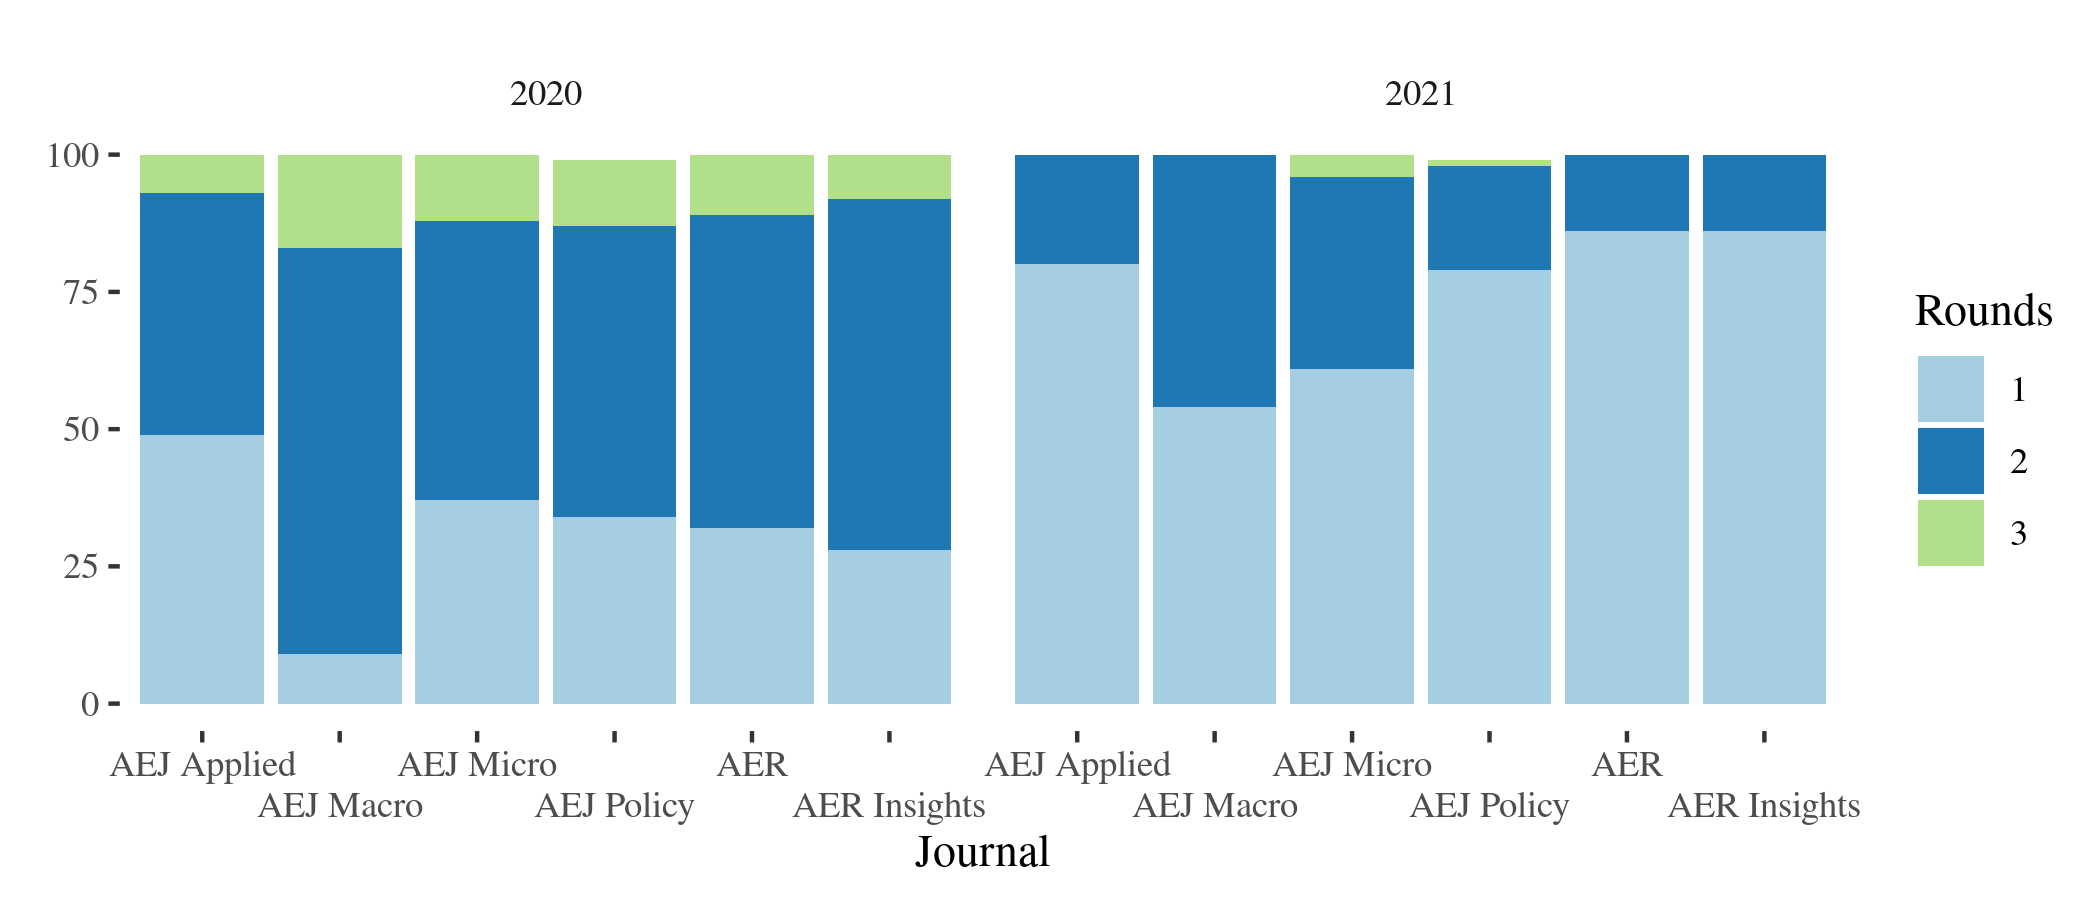
\includegraphics[width=\textwidth]{images/plot_rounds_compare.png}
    \centering
    \caption{Comparing rounds per journal between 2020 and 2021\label{fig:rounds}}
\end{figure}

\paragraph{Process improvements}

In order to increase the initial acceptance rate, we set out in Summer 2020 to review the entire process that authors face. We made several changes aimed at (a) providing authors with the information as early as possible, when it is still easy to include reproducible practices in projects at relatively low cost and (b) providing authors with better information, to reduce frictions and uncertainty. 

As noted  \hyperref[sec:dcap]{earlier}, we introduced informational forms upon submission, and a new short form, requested upon conditional acceptance, collecting salient information about the replication package.%
\footnote{These forms can also be found at \href{https://www.aeaweb.org/journals/data}{aeaweb.org/journals/data}.} 
Each of these forms has   links to updated and detailed guidance on how to prepare and submit replication packages. We also provide links to the reproducibility checks that our team uses, so authors know in advance what checks will be applied to their replication package. These changes were first rolled out in September 2020, and revised in June 2021. In addition, a template ``README'' \citep{READMEv1.0.0} was introduced in December 2020 as a joint effort with other data editors, helping to clarify the necessary information, and to provide structure to authors' efforts to document their processes.

\paragraph{Computational Infrastructure}

Most replication packages are computationally verified by replicators on the computers available to the Data Editor at the Cornell University Economics Department and the ILR School. The majority are handled on the Windows Server systems of the Cornell Center for Social Sciences, while some are run on the Linux-based Bioinformatics cluster. Occasionally, personal macOS laptops are used. Systems can handle memory requirements up to 1024 GB or up to 100 cores. 

While these systems are fairly standard, they cannot cover all scenarios described in authors' computational requirements. Furthermore, these systems, much like the authors' own systems, are not shareable more broadly, and thus sometimes make it difficult to control for specific requirements, or to share error messages in the most reproducible way.  

Increasingly, we have therefore explored and documented additional computational environments. We have used \curlcite{https://codeocean.com}{CodeOcean} \citep{clyburne-sherin2019} both to share active (but only partially successful) reproduction efforts and to publish reproducible ``capsules.'' We have also explored the use of ``WholeTale'' \citep{chard2020a}, collaborating with its maintainers and other reproducibility institutions (e.g., the Odum Institute, which conducts reproducibility checks for various political science journals) to expand the utility of the system for the social sciences. Both {{CodeOcean}} and WholeTale rely on containerization, often known under the commercial name ``Docker,'' which can be independently used to precisely define and then share computational environments. We have used containers directly in some instances, including with licensed software (Gurobi, Stata, geocod.io) and when data assets are too large to be accepted into either CodeOcean or WholeTale, running such containers on the Linux systems at Cornell University. Table~\ref{tab:containers} lists some recent examples. Sample code that is used by AEA replicators and can be used freely by any researcher can be found at the \purlcite{https://github.com/AEADataEditor/}{AEA Data Editor's Github repository} A more expansive overview of containerization issues in economics can be found at \citet{aeadataeditor2021}. 

We plan to continue exploring novel computational tools, their utility in accelerating and streamlining the verification process, and their availability for use for more efficient replication packages in economics.


\begin{table}
	\centering
	\caption{Use of containerization for replication packages}
	\label{tab:containers}
	\begin{threeparttable}
		\centering
		\begin{tabular}{@{\extracolsep{5pt}} ll} 
			\toprule 
			Replication package & Technology \\ 
			\midrule 
			\citet{rossi2021capsule,rossi2021data} & CodeOcean, Docker, Matlab\\
			\citet{dellavigna2021capsule,dellavigna2021data} & CodeOcean, Docker, Stata\\
			\citet{aeadataeditor2021a,dinkelman2022data} & Docker, Stata\\
			\citet{aeadataeditor2021b,brunnermeier2021}  & Docker, R \\
			\citet{assuncao2021capsule} & CodeOcean, R \\
			\bottomrule 
		\end{tabular} 
		
		\begin{tablenotes}
			\item[] \textit{Notes:} 
		\end{tablenotes}
	\end{threeparttable}
\end{table}




\subsection{Archive for Replication Packages}

The default archive for replication packages accompanying articles in AEA journals is the \aeadcr{}. Deposit instructions are provided on the Data Editor's website, and mentioned upon conditional acceptance. However, it is not the only acceptable archive, as we discuss below.

The default allowed package size is 30GB. In the past year, the median package size was  \pkgsizemedian{} MB, but a significant number of packages (\pkgsizetwog{} percent) had  packages larger than 2GB. The move to a larger default size significantly reduced hurdles for authors.   \pkgsizetwentyg{} percent of deposits were larger than 20GB. Some packages have more than 1,000 files, hitting a technical constraint. Provision of opaque ZIP files are generally prohibited. Instructions on how to proceed when file numbers are large, while maintaining maximum visibility onto the file and package structure, are provided on the website. Authors with large packages, or packages with more than 1,000 files, should contact the AEA Data Editor. Depositing at other trusted repositories is one option, described in the next section.


%\subsection{Migrating Historical Supplements}
%\label{sec:migration}
%
%We  migrated the bulk of historical data (and code) supplements in 2019, from ZIP files stored on AEA servers to the \aeadcr{}. A few dozen replication packages are still awaiting migration. Most of these packages either have a very large number of files that surpass technical limitations of the \aeadcr{}, or turned out to be corrupted or illegible in their original version. We are still working on migrating these as resources permit. 
%
%% report on UMich metadata project
%% data provided by email
%
%We reported last year on a project with a research team at the University of Michigan, which solicited metadata improvements to migrated replication packages.  911 researchers provided additional metadata for 522 studies, which were incorporated into the \aeadcr{} in October 2021. We are currently assessing the impact of the improved metadata on findability of such packages.



\begin{figure}[t]
    \centering
    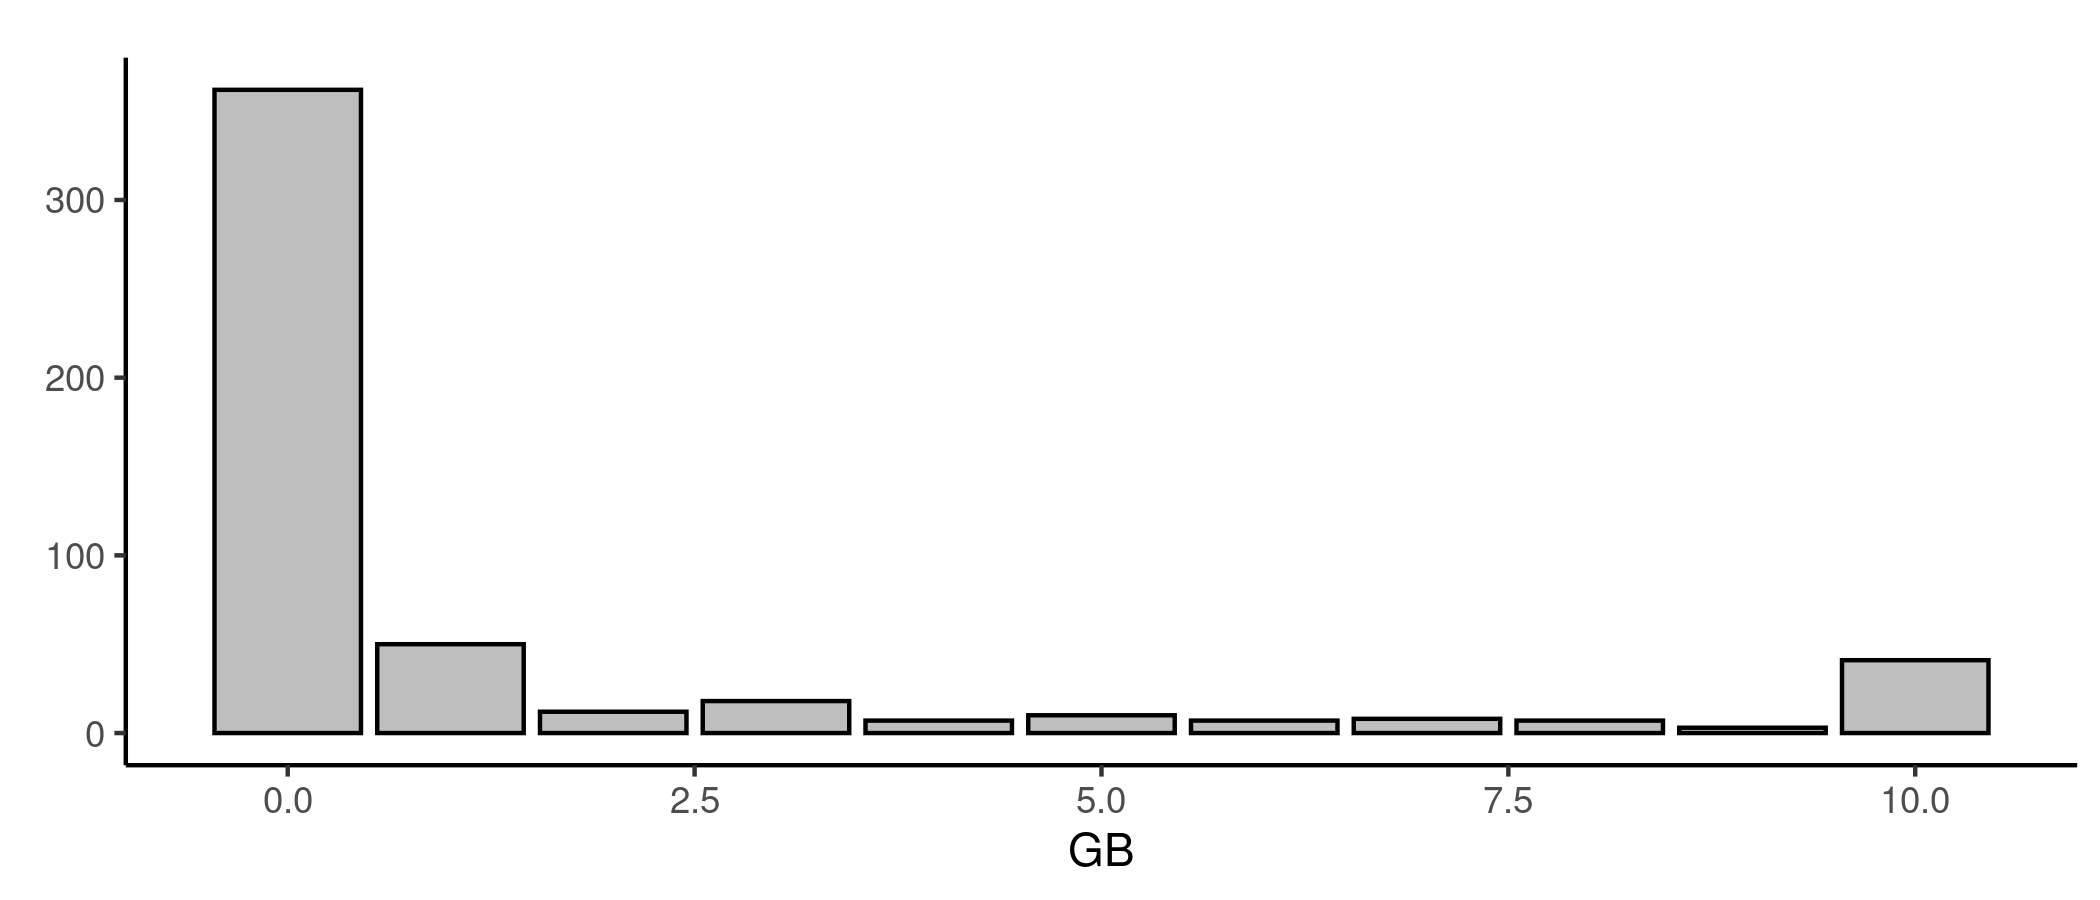
\includegraphics[width=\textwidth]{images/plot_filesize_dist.png} 
    \caption{Size distribution of replication packages deposited between  \firstday{} to \lastday{}, top-coded at 10GB.}
    \label{fig:size_packages}
\end{figure}


\subsection{Third-party repositories}

The \ac{DCAP} allows for code and data  to be deposited at other trusted repositories, as long as all other elements of the \ac{DCAP} are complied with. In fact, authors are \textit{discouraged} from duplicating deposits they have made elsewhere. This is intended to allow authors to create replication packages prior to submitting at the AEA's journals, or any other journal, as a component of a reproducible workflow and possibly in compliance with funder data management policies. Only a few authors have availed themselves of this option, depositing or referencing materials in particular at the \urlcite{https://dataverse.harvard.edu/}{Harvard Dataverse} and \purlcite{https://zenodo.org/}{Zenodo} To support authors depositing on Zenodo, we have created a ``Zenodo community'' at \href{https://zenodo.org/communities/aeajournals/}{zenodo.org/communities/aeajournals/}. At this time, examples include \citet{caroline_fohlin_2021_5151203}, who deposited code and data for their P\&P paper, and \citet{gendron_carrier_nicolas_2020_4317553}, whom we helped deposit data that was too cumbersome to deposit on ICPSR infrastructure ($>$ 200GB).%
\footnote{Code to support uploading large quantities of data to Zenodo via the Zenodo API, originally created by LDI Lab Member Vansh Gupta, can be found at \href{https://github.com/AEADataEditor/Upload-to-Zenodo}{github.com/AEADataEditor/Upload-to-Zenodo}.} 
Additional Zenodo deposits are currently being prepared for publication in 2022. Third-party repositories are linked to the main \aeadcr{} deposit, and are cited in the main article when appropriate. Authors wishing to deposit replication packages early in the research lifecycle are encouraged to consult the \curlcite{https://social-science-data-editors.github.io/}{Social Science Data Editors website} where links to trusted repositories are provided.  


\section{Working with Other Providers of Scientific Infrastructure to Improve Support for Documenting Provenance and Replicability}
\label{sec:coordination}

An important responsibility of the AEA Data Editor is to interact with other providers of scientific infrastructure. This includes other publishers and journals, archives such as ICPSR, providers of restricted or proprietary data, the AEA RCT Registry, metadata harvesters, and third-party verification services. 

\subsection{Highlighting and Preserving Data Resources}

We identified Zenodo as a possible solution to preserving large-scale data resources. By creating the ``AEA Zenodo Community,'' we are able to highlight data resources that have, in the past, often not been curated or preserved appropriately. In addition to very large data resources, we also occasionally work to preserve data resources created by the U.S. government, used in multiple articles, but not formally preserved elsewhere. This includes \citet{SEER2021,BRFSS2021a,BRFSS2021b,SMARTBRFSS2021}. As needed, these will be updated. 


\subsection{Data Providers}
\label{sec:producers}

We regularly meet and communicate with academic, governmental, and commercial data providers, on behalf of specific authors or because we have identified a data provider as a frequently used resource. Discussion topics include making data citations easier, clarifying licenses, requesting blanket or streamlined data redistribution authorizations, or suggesting improved data curation practices to avoid repeatedly copying data from uncurated websites to the curated \aeadcr{}. 

In the course of the past year, we have talked about some or all of these topics with IPUMS, the World Bank, Standard and Poor's, the Federal Reserve of St. Louis data librarians, John Abowd, Rob Sienkiewicz, and Barbara Downs (U.S. Census Bureau), Philipp vom Berge and Dana Müller at the Research Data Centre (FDZ) of the German Federal Employment Agency (BA) at the Institute for Employment Research (IAB), Paulo Guimarães at the \ac{BPLIM}, Ricardo Dahis (Base dos Dados, \href{https://basedosdados.org/}{basedosdados.org}), and Kamel Gadouche and Roxanne Silberman at the French \textit{Centre d'accès sécurisé de données} (CASD). We have also talked to various research groups on how to improve data curation, visibility, and citability of the data created by their efforts.

\subsection{Economics Journals}

We continue to coordinate with other data editors conducting similar activities at other journals. An informal mailing list managed by the AEA Data Editor is used to interact with others.\footnote{Journal editors are encouraged to join the mailing list by contacting the AEA Data Editor.} Mailing list members who wish to be more actively involved can participate in the development of the \purlcite{socialsciencedataeditors.github.io}{website of the Social Science Data Editors} The website contains guidance on data citations and data availability statements, best practices for coding and data preparation, and links to various tools useful to replicators. The authors of the template README, Lars Vilhuber, Miklos Kóren (\acl{ReStud}), Joan Llull (\acl{EJ}), Peter Morrow and Marie Connolly (\acl{CJE}), continue to collect input on improvements on the README, and expect to have an updated and improved version available in 2022. The Data Editor has also been invited to the Steering Committee of a group of data repository leaders at Data-PASS organized as the Journal Editors Discussion Interface (\urlcite{https://dpjedi.org/}{JEDI}).


\subsection{Third-party verification services}
\label{sec:3rdparty}


We continue to rely on and have discussions with third-party verification services. As noted earlier, \jiraexternal{} reports were provided by external replicators or replication services for \jiramcsexternal{} manuscripts (see Table~\ref{tab:jirastats} for statistics by journal, Appendix~\ref{app:3rdparty} for a list of third-party replicators). 

\section{Working with the Economics Community to Enhance and Broaden Education on Replicable Science}

Outreach through presentations and publicly available tools is a key component of an effective data and code availability policy. 

\subsection{Presentations}

The Data Editor participated in the \ac{CSWEP} ``\urlcite{https://www.aeaweb.org/about-aea/committees/cswep/programs/resources/webinars}{Fireside chats}'' on January 19, 2021 with the topic ``Demystifying Replication Requirements and Processes: Best Practices Viewed by AEA Data Editor.'' Presentations on reproducibility in economics, and the various efforts surrounding the \dcap{}, have been presented at the NSF Webinar on Best Practices in Making Research Datasets Publicly Accessible, the Research Data Alliance's \href{https://www.rd-alliance.org/rdas-17th-plenary-meeting-programme}{17th Plenary}, a CNSTAT Expert meeting on Guidance on Data Sharing for NIA Longitudinal Studies, the Future of Privacy Forum Promoting Responsible Research Data Access, and at workshops at the IAB, CES-ifo, NBER, and Banco de Portugal. Recordings of  presentations (when available) and presentations materials are listed at the \purlcite{https://aeadataeditor.github.io/talks/}{Data Editor's website} Together with BITSS (UC Berkeley), a framework and platform to support teaching reproducibility is being developed, called the ``Social Science Reproduction Platform'' (\href{https://www.socialsciencereproduction.org/}{www.socialsciencereproduction.org}), complementing other existing services such as the ReplicationWiki. The platform has been presented at CTREE 2021 and the ASSA 2022 meetings. A paper on the education and training of undergradudate replicators is under review at the \textit{Journal of Statistics and Data Science Education} as of January 1, 2022.

\subsection{Resources}

The AEA Data Editor maintains public resources available to the economics community. These are made available through a dedicated website at \href{https://aeadataeditor.github.io/}{aeadataeditor.github.io/} and code and project templates provided at \href{https://github.com/aeadataeditor}{github.com/aeadataeditor}. In particular:

\begin{itemize}
    \item Step-by-step guidance on how to prepare a replication package is provided at \href{https://aeadataeditor.github.io/aea-de-guidance/}{aeadataeditor.github.io/aea-de-guidance/}, including video tutorials and a description of the process. 
    \item The template README \citep{READMEv1.0.0} is referenced as part of the guidance, and separately accessible at \href{https://social-science-data-editors.github.io/template_README/}{social-science-data-editors.github.io/template\_README/}.
    \item Various blog posts on topics relating to computational reproducibility are posted at \href{https://aeadataeditor.github.io/year-archive/}{aeadataeditor.github.io/year-archive/} and typically summarized on Twitter under the Data Editor's handle \href{https://twitter.com/AEAData}{@AEAData}.
    \item Instructions to replicators for assessing authors' replication packages are provided at \href{https://github.com/AEADataEditor/replication-template}{github.com/AEADataEditor/replication-template}.
    \item Template code for using containers for Stata, R, Julia, and Gurobi can be found by \href{https://github.com/AEADataEditor?q=docker&type=all&language=&sort=}{searching for ``docker`` on the Github site}.
    
\end{itemize}


\section{Replication team at Cornell University}

\subsection{Replicators} 
\label{app:replicators}

The following \textbf{\teamsize} students have provided excellent assistance in reproducing the results from the \jiramcs{} articles processed by the Replication Lab:
%
% Pulled from processing-jira...
%
%
Andreas Psahos,
Asha Patt,
Ashley Cooray,
Craig Schulman,
Daniella Pena,
Dmitry Shlyapnikov,
Eli Kolodezh,
Emma Sbrollini,
Hongyi Duan,
Huey Le,
Jacob Recht,
Jaeyoung Shim,
Janet Malzahn,
Jared Martin,
Jill Crosby,
Jonathan Temkin,
Joshua Passell,
Julia Zimmerman,
Kate Hofer,
Kevin Bao,
Liam Cushen,
Lilly Thomalla,
Lincy Chen,
Lydia Reiner,
Matt Wang,
Matthew LaFontaine,
Melanie Brown,
Melanie Chen,
Miranda Zhou,
Nehedin Juarez,
Ololade Omotoba,
Qianyi Liu,
Ryan Ali,
Sam Evans,
Satya Datla,
Steve Yeh,
Surita Basu,
Suvd Khaliun,
Tarangana Thapa,
Taren Daniels,
Vansh Gupta,
Xiangru Li,
Zebang Xu,
Zechariah Karsana.



Graduate students Hyuk Harry Son and Leonel Borja Plaza  and Research Aide Michael Darisse (all Cornell University) have been invaluable assistants in training and coordinating the work as well as developing the methods and procedures which we have made public. Leonel Borja Plaza contributed programming to this report. 

\subsection{Computing support}

We thank the Economics Department and the ILR School for providing us with computing resources at the Cornell Center for Social Sciences and the Bioinformatics cluster. 

\section{Third-party contributors}

\subsection{Replicators}
\label{app:3rdparty}

We are grateful to the following third-party replicators, who assisted us with verifications when we were unable to access data or, in some cases, computing resources. We do not name individuals when doing so would reveal information not already known to the manuscript's authors, naming the institution instead. Names are listed in no particular order.
%
Daniel Feenberg (\ac{NBER}), Karma Sonam and Keenan Dworak-Fisher (both \ac{BLS}), Paulo Guimarães (\ac{BPLIM}), Lisa Neilson and Joshua Hawley (\ac{OLDA}), Philipp vom Berge (IAB), Ian Schmutte (UGA) graduate students Caitlin Ahearn (UCLA), Manuel V. Montesinos (Universitat Autònoma de Barcelona, on behalf of the Data Editor of the Economic Journal, Joan Llull)   We in particular want to again thank Olivier Akmansoy, Christophe Hurlin (Université d'Orléans), and Christophe Pérignon (HEC Paris), all of \href{https://cascad.tech}{cascad}, a certification agency for scientific code and data, who have been generous of their time and resources, and have provided us with 4 reports during this time.  

We do not name the authors with whom we signed non-disclosure agreements, or who otherwise provided us with access to data that could not be published. We are grateful for their flexibility and patience.

\subsection{Computing resources}
\label{app:3rdparty-computing}

We are grateful to CodeOcean, NBER, WholeTale, and Harvard Business School, who all provided us with access to computing resources at no cost, and technical assistance when necessary. We use free academic resources on Github and Bitbucket. 


\section{Disclosures}
\label{sec:disclosure}

We received a generous compute and storage quota from \href{https://codeocean.com/}{CodeOcean}, a free license to use Stata 17 for one year in cloud applications from \href{https://stata.com/}{Stata}, and a subaward on NSF grant \href{https://nsf.gov/awardsearch/showAward?AWD_ID=1541450&HistoricalAwards=false}{1541450} ``CC*DNI DIBBS: Merging Science and Cyberinfrastructure Pathways: The Whole Tale'' from the University of Illinois to evaluate the WholeTale platform for the purpose of reproducibility verification. None of the sponsors have reviewed this preliminary assessment, or have had influence on any of the conclusions of this document. CodeOcean currently offers academic users a certain number of monthly free compute hours. WholeTale is free to use,  the Stata  functionality mentioned here is expected to be available in early 2022.


\section{Data and Code Availability Statement}
\label{sec:dcas}

All publicly available data and code used to generate figures and tables in this article are available \citep{report2021data,E117876V3}. Some detailed data from the editorial system, used for Table~\ref{tab:pre:rounds}, are considered confidential and cannot be made available in a way that preserves the privacy of the editorial process at this time.

\begin{flushright}
{\sc Lars Vilhuber}, \textit{Data Editor}
\end{flushright}


\FloatBarrier
% Remove or comment out the next two lines if you are not using bibtex.
%
% NOTE: Do not modify the AEADataEditor.bib manually!
%
\bibliographystyle{aea-mod}
\bibliography{paper,references,refs-zotero}

% The appendix command is issued once, prior to all appendices, if any.
\appendix

%\input{appendix.tex}


\end{document}

